\documentclass{standalone}
\usepackage{amssymb}
\usepackage{tikz}
\usetikzlibrary{arrows.meta}
\usetikzlibrary{shapes.geometric,arrows,positioning}

\begin{document}

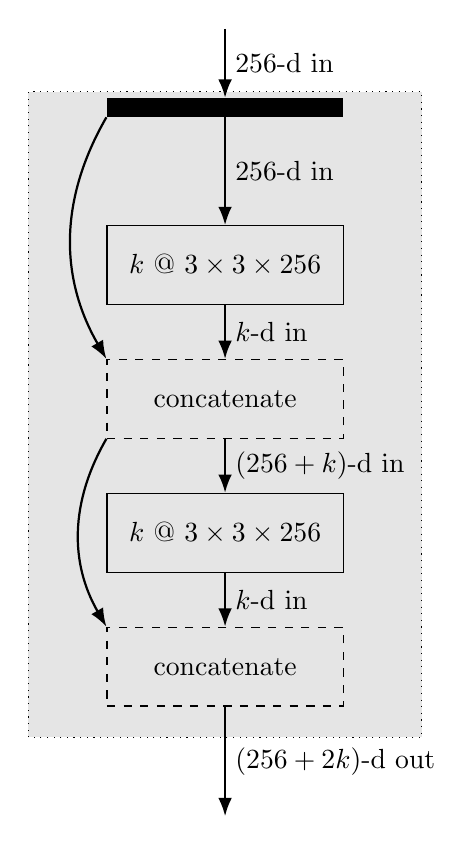
\begin{tikzpicture}
    \tikzstyle{conv-layer}=[draw,minimum width=3cm,minimum height=1cm]
    \tikzstyle{arrow}=[->, -Latex, thick]

    \draw[fill=black!10,dotted] (-2.5, -7.0) rectangle (2.5, 1.2);

    \node[rectangle, fill=black,minimum width=3cm] (input) at (0, 1) {};
    \path[arrow] (0, 2) edge node[right, midway] {$256$-d in} (input.north);

    % first path
    \node (conv1) at (0,-1.0) [conv-layer] {$k$ @ $3 \times 3 \times 256$};
    \node (conc1) at (0,-2.7) [conv-layer, dashed] {concatenate};
    \node (conv2) at (0,-4.4) [conv-layer] {$k$ @ $3 \times 3 \times 256$};
    \node (conc2) at (0,-6.1) [conv-layer, dashed] {concatenate};

    \path[arrow] (input.south) edge node[right, midway] {$256$-d in} (conv1.north);
    \path[arrow] (conv1.south) edge node[right, midway] {$k$-d in} (conc1.north);
     \path[arrow] (conc1.south) edge node[right, midway] {$(256 + k)$-d in} (conv2.north);
    \path[arrow] (conv2.south) edge node[right, midway] {$k$-d in} (conc2.north);

    \path[arrow] (input.south west) edge[bend right] node[right, midway] {} (conc1.north west);
    \path[arrow] (conc1.south west) edge[bend right] node[right, midway] {} (conc2.north west);

    \path[arrow] (conc2.south) edge node[right] {$(256+2k)$-d out} (0, -8);

\end{tikzpicture}
\end{document}
